While providing exhaustive descriptive analysis for every features is not feasible within this short report, given their diversity, the reader can refer to the companion notebook. In this section, we focus on analyzing the spatio-temporal coverage of our dataset, as it is important for the rest of the discussion.

\begin{figure}[!h]
	\centering
	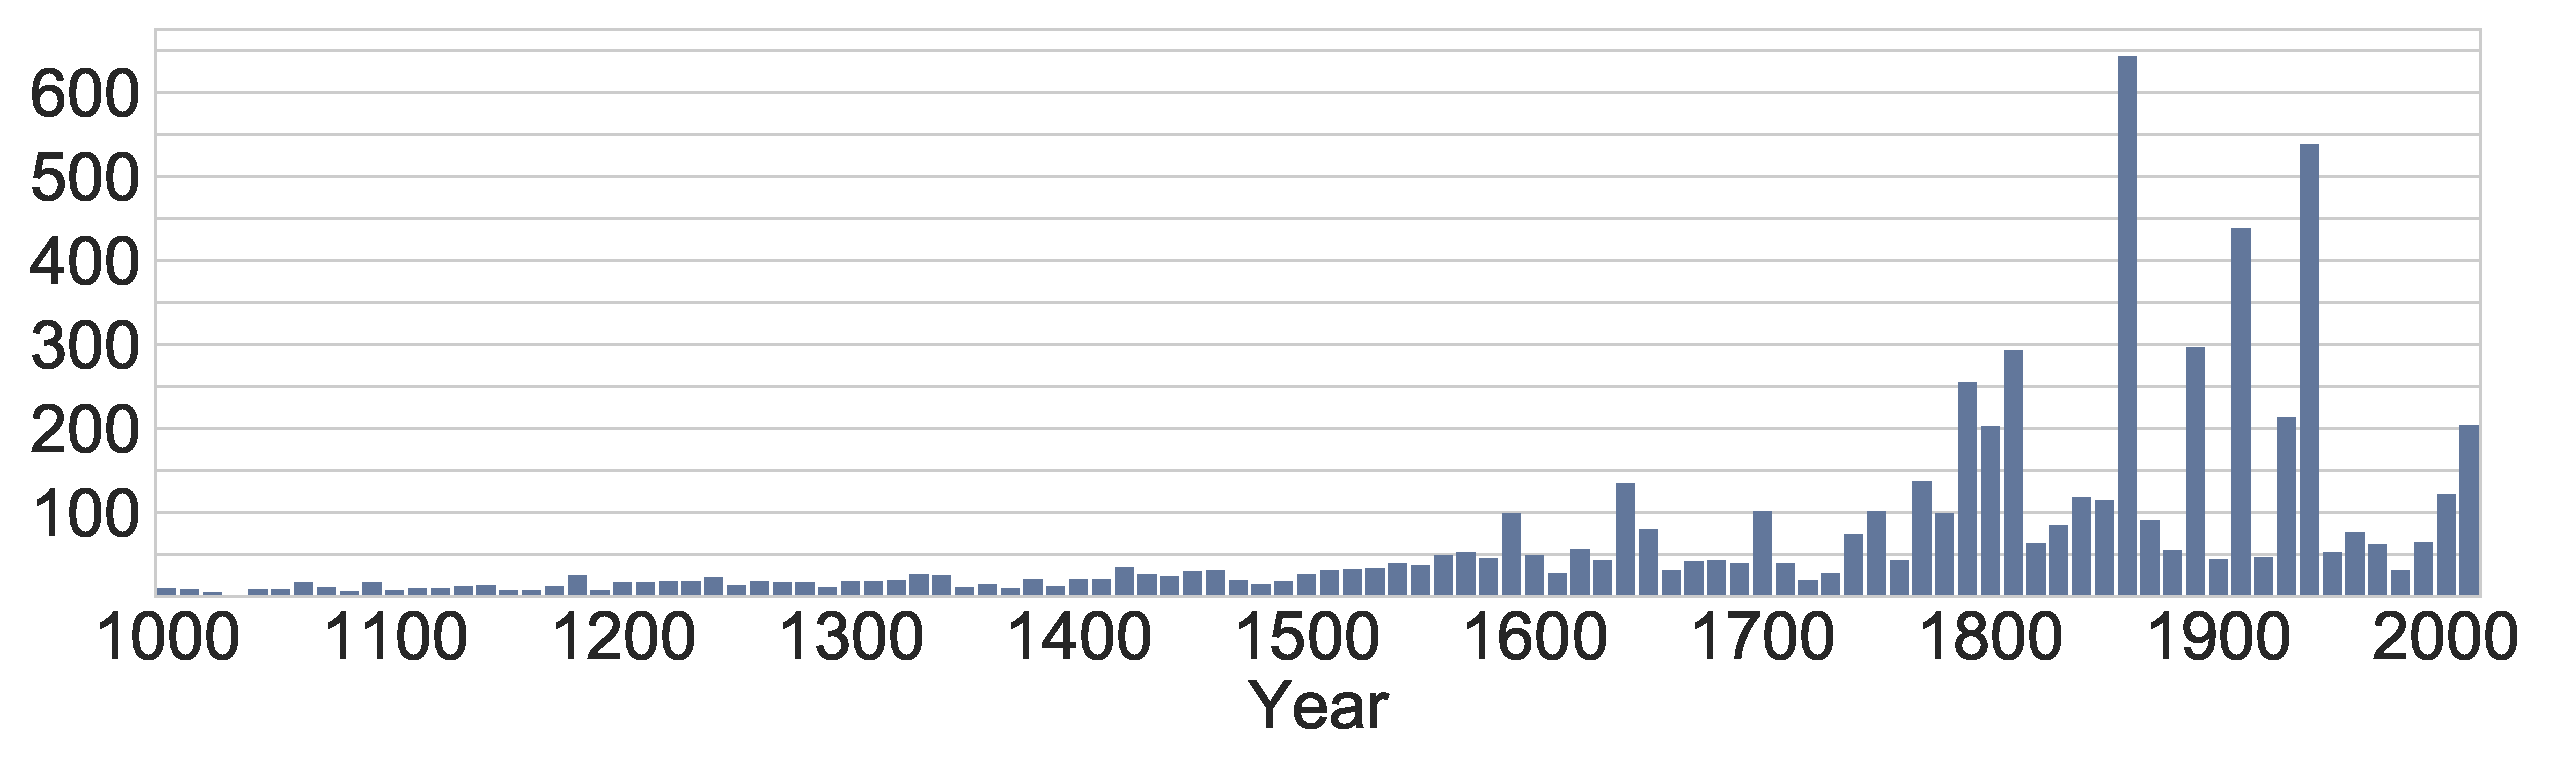
\includegraphics[width=\linewidth]{figures/temporal_coverage.eps}
	\caption{Battle count per decade}
	\label{fig:temporal_coverage}
\end{figure}

\begin{figure*}[!t]
	\centering
	\begin{subfigure}[b]{0.495\linewidth}
		\centering
		\includegraphics[width=\linewidth]{figures/1000-1700.png}
		\caption[]%
		{{\small 1000 --- 1700}}    
		\label{fig:geodens_1000-1700}
	\end{subfigure}
	\begin{subfigure}[b]{0.495\linewidth}  
		\centering 
		\includegraphics[width=\linewidth]{figures/1700-1900.png}
		\caption[]%
		{{\small 1701 --- 1900}}    
		\label{fig:geodens_1700-1900}
	\end{subfigure}
	\vskip0.2\baselineskip
	\begin{subfigure}[b]{0.495\linewidth}   
		\centering 
		\includegraphics[width=\linewidth]{figures/1900-2000.png}
		\caption[]%
		{{\small 1901 --- 2000}}    
		\label{fig:geodens_1900-2000}
	\end{subfigure}
	\begin{subfigure}[b]{0.495\linewidth}   
		\centering 
		\includegraphics[width=\linewidth]{figures/2000-2018.png}
		\caption[]%
		{{\small 2001 --- 2017 }}    
		\label{fig:geodens_2000-2017}
	\end{subfigure}
	\vskip0.2\baselineskip
	\caption{\small Geographic density of battles for different year ranges.} 
	\label{fig:geodens}
\end{figure*}

We first look at the distribution of events in time in Figure \ref{fig:temporal_coverage}. Peaks are clearly observable during the American Civil War, the first and the second World Wars,  while the years 1000 to 1700 have low battle counts per decades. Notice that this does not mean they were more peaceful, only that less battles were recorded.

Then, we display the geographic distribution for chosen periods and as we can see in figure \ref{fig:geodens}, battles were occurring mostly in Europe between the $11^{th}$ and the $17^{th}$ centuries. The $18^{th}$ and the $19^{th}$ centuries are the only ones in which many battles occurred on the North American continent (with the 1861 Civil War), these centuries also witnessed the First Opium and Sino-Japanese Wars in Asia. 